\documentclass[10pt]{article}
\usepackage{amsfonts}
\usepackage{amsmath}
\usepackage[font=small,labelfont=bf]{caption}
\usepackage{fancyhdr}
\usepackage[margin=1.0in]{geometry}
\usepackage{graphicx}
\usepackage{hyperref}
\usepackage{multicol}
\usepackage{textcomp}
\setlength{\columnsep}{0.5cm}
\setlength{\headheight}{24pt}
\setlength{\parindent}{15pt}
\pagestyle{fancy}
\fancyhf{}
\lhead{
	CSE 847: Machine Learning---Final Report \\
	Langford, Lingg, and Lucero
}
\rhead{April 28, 2017}
\cfoot{\thepage}
\begin{document}
	\title{
		CSE 847: Machine Learning---Final Report \\
		\textbf{An Exploration and Implementation of Automated Valuation Models to Learn and Predict the Value of Real Estate}
	}
	\author{
		\begin{tabular}{ccc}
			Mick Langford & Mike Lingg  & Jordi Lucero \\
			langfo37@msu.edu & linggmic@egr.msu.edu & luceroj2@msu.edu \\
			\textit{Neural Network} & \textit{Linear/Logistic Regression} & \textit{Decision Trees}
		\end{tabular}
	}
	\date{April 28, 2017}
	\maketitle
	\begin{multicols}{2}
		\section{Problem Description}
		Automated Valuation Models (AVM) have become increasingly popular as the real estate market has embraced the World Wide Web as a source of accurate, up to the minute data.\textsuperscript{\cite{kaggleblog}} Banks have also shown great interest in using AVMs to help mitigate fraud by human appraisal.\textsuperscript{\cite{scotsman}} Our goal is to explore various machine learning techniques to implement an AVM and predict the true value of a house based on features commonly found on real estate listings. Our data will be drawn from various datasets, including from the Nashville, TN housing market, using a dataset posted on Kaggle\textsuperscript{\cite{nashville_data}}.
		
		We have implemented both linear and logistic regression models that take into account physical attributes of each house and location. We have also implemented nonlinear models, such as decision trees and neural networks for comparison.
		
		\section{Related Work}
		An obvious and popular example is Zillow's proprietary Zestimate\textsuperscript{\textregistered}. Zillow uses a closed source AVM that takes into account special features of the home, location, and market conditions. Zillow admits to using features such as physical attributes, tax assessments, and prior transactions. Zillow claims to have data on 110 million homes and estimates on approximately 100 million homes.\textsuperscript{\cite{zillow}}

		Relevant papers include the doctoral dissertation of Lowrance which explores and compares various linear models on housing data for the Los Angeles County.\textsuperscript{\cite{lowrance}} Park and Bae explore machine learning algorithms such as C4.5, RIPPER, Naive Bayesian, and AdaBoost.\textsuperscript{\cite{park}} Bin performed a study that estimates a hedonic price function using a semi-parametric regression.\textsuperscript{\cite{bin}} This may be particularly useful for real estate listings that are incomplete or for data that is entered erroneously. Bourassa et al. consider the spatial dependence of house prices, which is intuitively an important factor.\textsuperscript{\cite{bourassa1}\cite{bourassa2}} Kauko et al. research neural network models to help investigate segmentation in the housing market of Helsinki, 
		
		Finland.\textsuperscript{\cite{kauko}} Azadeh et al. present an algorithm based on fuzzy linear regression and a fuzzy cognitive map to handle uncertainty in the housing market and improve the analysis of housing price fluctuations.\textsuperscript{\cite{azadeh}} Fan et al. introduce a decision tree approach for modeling and predicting house prices.\textsuperscript{\cite{fan}}

		\section{Project Data}
		Multiple sources of real housing sales data are considered for this project

		\textbf{Nashville Housing Data} The Nashville housing dataset is a list of home sales in the Nashville, Tennessee area, provided by Kaggle\textsuperscript{\cite{nashville_data}}. This dataset includes 29 fields of data for 56635 entries. However, nearly half of the entries have gaps in information, which will have to be accounted for.

		\textbf{King County Housing Data} The King County housing dataset is a list of home sales in the King County, Washington area, provided by Kaggle\textsuperscript{\cite{kc_data}}. This dataset includes 20 fields of data for 21614 entries, with none of the entries missing any data.
		\par
		\textbf{Advanced Regression Techniques Data} The Advanced Regression Techniques data is a list of home sales, provided by Kaggle. This data includes 79 features of housing data for 1460 homes. The data has no gaps, except for some N/A data.
		\par
		\textbf{Grand Rapids Data} The Grand Rapids data is a list of home sales in the Grand Rapids area, provided by the real estate listing service Redfin. This data includes 16 fields for 9646 entries. The dataset also has gaps in information for about half of the entries.
		\par
		The different datasets provide a variety of input to test machine learning techniques against. Data with more features should provide more accurate results, if the additional features provide useful information for the prediction.
		
		\section{Preprocessing Data}
		Prior to processing the data with our models, each dataset is first normalized by dividing each feature value by the difference between that feature's maximum and minimum values. The target sales prices are normalized across all datasets to allow for comparison of the model's performance. One issue considered is how to properly manage fields containing categorical values. Our approach is to treat a field with \(n\) categories as \(n\) binary features, indicating whether that entry is of the associated category or not. Finally, since some of our datasets are incomplete, different methods of substituting missing values are considered, such as using the feature mean, substituting values from the closest neighbor by way of Euclidean distance, or using the mean value from a group of closest neighbors.

        Table \ref{table:linr_preprocessing} shows the results of data preprocessing with a simple closed form linear regression, using the Advanced Regression Techniques Data. First, the data is considered with no preprocessing, with exception to the sale prices, which are normalized so that Mean Squared Error (MSE) can be compared between the results. Second, both the features and home prices are normalized. Third, in addition to normalization, all categorical features are split into a number of binary features for each categorical value. The observed results confirm that each additional method of preprocessing improves the MSE significantly. As a result of this analysis, the decision was made to preprocess all of our data by normalizing the values and splitting categorical features into binary.
        
		Basic closed form linear regression cannot be solved without either discarding entries with missing values or using some method of substitution. Table \ref{table:linr_hole_fill} provides a comparison of the methods considered for replacing missing values. These results are from applying closed form linear regression to the Grand Rapids dataset from Redfin. Using the mean value of the missing features is a valid option but is not ideal. To improve upon this, each member in the set of incomplete entries is compared to those that are complete, computing the Euclidean distance between the known values of each incomplete entry. The corresponding values in the nearest complete entry to each incomplete entry is used as a substitute. This method demonstrated an improvement in observed MSE from linear regression. However, an even greater improvement is found when instead of just using the values from the closest neighbor to each incomplete entry, the mean values from the ten closest neighbors is used instead. This final method of substitution should be assumed for all of the models discussed in this report.
		\begin{center}
			\captionsetup{type=table}
			\begin{tabular}{l|c}
				Feature Preprocessing & \small{MSE} \\
				\hline
				\small{None} & \small{1.2487} \\
				\hline
				\small{Normalization.} & \small{0.0499} \\
				\hline
				\small{Binary Features} & \small{0.0012} \\
			\end{tabular}
			\captionof{table}{MSE for preprocessing techniques.}
			\label{table:linr_preprocessing}			
		\end{center}

		\begin{center}
        	\captionsetup{type=table}
			\begin{tabular}{l|c}
				Substitution Method & \small{MSE} \\
				\hline
				\small{None} & \small{---} \\
				\hline
				\small{Mean} & \small{1.6e-3} \\
				\hline
				\small{Closest Value} & \small{1.2e-3} \\
				\hline
				\small{Closest Mean} & \small{1.1e-3} \\
			\end{tabular}
			\captionof{table}{MSE for missing value substitution.}
			\label{table:linr_hole_fill}
		\end{center}

        During the course of research, the MSE measured by our models was observed to be producing greatly different results between datasets. Models that appeared to produce a good match were resulting in higher error than models that appeared to produce weaker results. It was observed that the datasets producing lower error had more lower-valued houses and few high-valued. This issue was addressed by filtering out any homes with sales prices above \$1M, in order to eliminate these boundary cases. Outliers were pruned prior to missing value substitution, to ensure that the pruned entries has no influence on substituted values. Additionally, the target sales prices were normalized across all datasets to ensure that the MSE computed by each model for each dataset could be compared.
 		\section{Models}
		\subsection{Linear Regression}
			For linear regression we are using a closed form ridge regression. We tested standard and stochastic gradient descent but these methods did not produce a significant improvement in processing time for the data we are using, and do not improve on the prediction error.
		\par
			For the ridge regression regularization value we developed a simple automated approach to identify the ideal regularization value. We start with a test regularization value of 1 and perform five fold cross validation on the training data to determine the mean square error with this test value. Then we adjust the test value by 0.1 in the positive direction, in this case moving from 1 to 1.1, and repeat the cross validation. If the error decreases, we continue to adjust the test value in the same way. If the error increases, we reverse the sign of the test value adjustment and divide it by 10. This is like a simplistic gradient descent, but when we overshoot the minimum we reverse direction and lower the step size. This continues until the error between two cross validations matches within 1e-7.
		\par
		\begin{center}
                  \captionsetup{type=figure}
			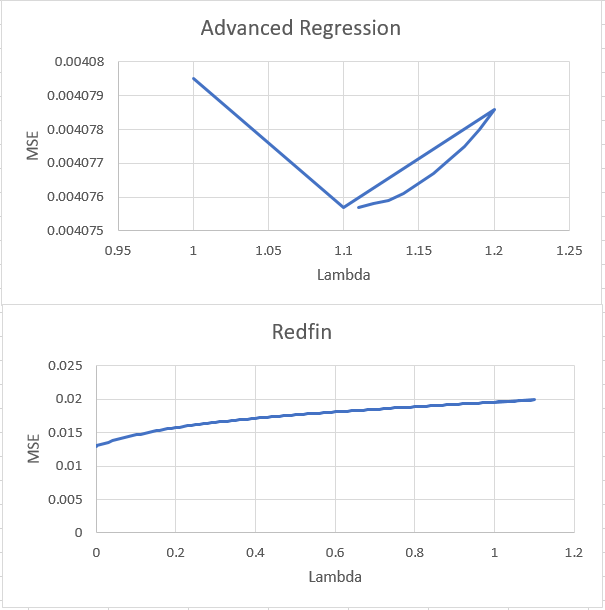
\includegraphics[scale=0.60]{Images/LinearRegressionCrossTrain} \\
			\captionof{figure}{Linear regression cross training.}
			\label{fig:linr_cross_train}
		\end{center}
		\par
                Figure \ref{fig:linr_cross_train} shows a sample of our cross training method on the Advanced Regression and Redfin datasets. The advanced regression data initially shows a reduced error when moving from 1 to 1.1 so it increases to 1.2.  At 1.2 the error goes back up again so it reverses direction and moves back in increments of 0.01, until it reaches a stable point. This shows a place where the algorithm works but could possibly have been made more efficient, but still works for our current purposes. The Redfin data starts at a regularization value of 1 but sees an increase of error at 1.1 so decreases at a lower rate. What can be seen in the data, but is not visible in the graph, is around 0.013 lambda the regularization search reverse direction, an dincreases precision, several times to find the minimum solution.
		\par
		Table \ref{table:linr_performance} shows the mean square error of linear regression for each dataset. As expected the advanced regression techniques dataset provides the least error as this data provides the most complete features for each house. Nashville performs the weakest as there are very large gaps in the data, which must be filled in by preprocessing. The interesting result is between Redfin and King's county data. King's county has the same number of features as redfin and more homes in the dataset. Preprocessing the data shows that the redfin features have more categories and the redfin house prices are concentrated more at the lower end, whereas the King's county features have few categories and have prices fairly evenly distributed over the normalized range. As a result, redfin has more information in the features and the prices are easier to predict, which appears to be what produces the lower error.
		\par
        	\captionsetup{type=table}
			\begin{tabular}{r|c}
				& \small{Mean Squared Error} \\
				\hline
				\small{Nashville} & \small{22.1e-03} \\
				\hline
				\small{Advanced Regression} & \small{1.0e-03} \\
				\hline
				\small{Redfin} & \small{6.3e-03} \\
				\hline
				\small{King's County} & \small{13.1e-03} \\
				\hline
			\end{tabular}
			\captionof{table}{Observed performance from linear regression model.}
			\label{table:linr_performance}        
			\setlength{\parindent}{15pt}
		\par
		We also tried two ensemble methods with linear regression. The first method divides the features into groups of 4, performs linear regression on each group and adds the group results together. Linear regression is then performed on the summation of the groups. The second method picks random groups of 10 features with 100 groups and then an ensemble is produced in the same method as the groups of 4 in the previous method. Additionally each ensemble method was tested with PCA feature reduction providing 25\%, 50\%, 75\% and 100\% of features. This method was tested against all of the datasets except for the Nashville data as an SVM on the Nashville data exceeded matlab's available memory.
        \par
        Figure \ref{fig:linr_ensemble} shows the results of the ensemble methods. The advanced regression techniques and King's county data performed close to the pure linear regression. The redfin dataset showed a slight improvement over linear regression.
		\begin{center}
                  \captionsetup{type=figure}
			\includegraphics[scale=0.6]{Images/LineEnsembleResults} \\
			\captionof{figure}{Linear regression ensemble results.}
			\label{fig:linr_ensemble}
		\end{center}
		\par
 		\subsection{Classification}
			We are also approaching this problem as a classification problem for our linear regression and neural network models. The range of sale prices for the entire dataset will be partitioned into \(k\) classes, each class can include the same range of values, or be variable in size to accommodate ranges with similar input data. The classification solutions will then be fitted to a training dataset, and finally predict each entry in the test dataset by fitting it into one of the \(k\) classes.
		\subsection{Logistic Regression}
			During initial logistic regression development, we have used two different approaches to perform classification.
		\par
			The first approach attempt to classify which of the k class ranges the house most likely falls in based on input data. This model is composed of a matrix of independent regression models. It is trained for each input data point by setting the Y value corresponding with the class the house value falls under to 1 and all others to 0. The current training method uses stochastic gradient descent with a reducing step size. Once trained, the logistic regression class with the most confident result for the given input data is the one under which we classify a house.
		\par
	 		The second approach also uses a matrix of independent regression models but instead the results classify if the house is worth more than the lower value of the class k of each model. The training method only differes from the first approach by setting the Y value corresponding with the class equal to 1 if the value of the current house is higher than the lower value of the class. Then classification is performed by summing up the range represented by each class with a confidence higher than 0.5.
		\par
 			Table \ref{table:logr_performance} shows a comparison using the Advanced Regression Techniques data of the linear regression vs the two logistic regression approaches. The table shows that the second approach for logistic regression, determining if the house is worth more than each class, works better than the first approach, determining which class the house would fall under.
		\par
        	\captionsetup{type=table}
			\begin{tabular}{r|c}
				& \small{Mean Squared Error} \\
				\hline
				\small{Linear Regression Model} & \small{1.0e-03} \\
				\hline
				\small{Logistic Regression Model 2} & \small{4.8e-03} \\
				\hline
				\small{Logistic Regression Model 1} & \small{13e-03} \\
				\hline
			\end{tabular}
			\captionof{table}{Observed performance from logistic regression model.}
			\label{table:logr_performance}        
			\setlength{\parindent}{15pt}
		\par
			Figure \ref{fig:logr_MSE_Accuracy} shows the accuracy is best for a small number of classes, except for Advanced Regression Techniques. For Advanced Regression Techniques, 5 classes causes most houses to fall right on a boundary between classes, which causes poor performance. Advanced Regression Techniques performs better for 10 classes, where most of the house values happens to fall into classes more evenly. While accuracy decreases with an increase in classes, the mean squared error difference between the lowest value of the predicted class and the true value decreases. This is caused by predictions being for a narrower range with more classes, increasing the precision.
		\par
		\begin{center}
	            \captionsetup{type=figure}
			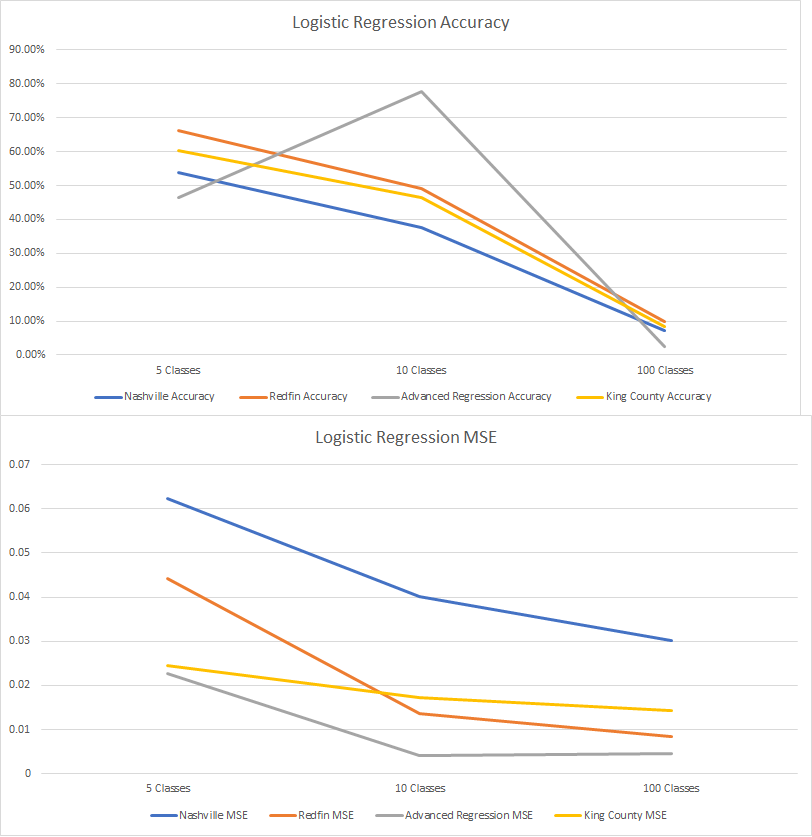
\includegraphics[scale=0.6]{Images/LogisticRegressionMSEAccuracy} \\
			\captionof{figure}{MSE and accuracy for Logistic Regression.}
			\label{fig:logr_MSE_Accuracy}
		\end{center}
		\par
			Finally we implemented an ensemble that performed linear regression on top of the logistic results. This ensemble used the 100 class logistic regression test predictions for training and testing. Similar to previous runs, the Nashville data was skipped as it produces too large of a matrix for matlab. As shown in table \ref{table:logr_ensemble}, the ensemble provides at least a small improvement on each dataset as compared to the base logistic regression.
		\par
        	\captionsetup{type=table}
			\begin{tabular}{r|c|c}
				& \small{Original Logistic} & \small{Ensemble} \\
				\hline
				\small{Redfin} & \small{8.5e-03} & \small{8.1e-03} \\
				\hline
				\small{Advanced Regression} & \small{4.5e-03} & \small{1.7e-03} \\
				\hline
				\small{King's County} & \small{14.4e-03} & \small{13.2e-03} \\
				\hline
			\end{tabular}
			\captionof{table}{Observed performance from logistic regression ensemble.}
			\label{table:logr_ensemble}        
			\setlength{\parindent}{15pt}
		\subsection{Decision Tree}
		\par
		For our Decision Tree approach, we used a Classification Decision Tree and a Regression Decision Tree. For the Classification Tree, since the data was not already classified, it was split into \(k\) equally sized classes where each class represents a range of prices. The average value for every feature column is also calculated and used to subsitute for any missing data points in the observations. A classification model was built for the KC dataset, Redfin dataset, and Nashville dataset. For each dataset, initially a classification tree model was built using crossfold validation with 10 folds using 90\% of the data for training. This model used the default parameters for tree size, which are maximum number of splits of n-1, minimum leaf size of 1, and minimum parent size of 1. 
		\par		
Another classification model was built by using 10 fold cross validation and generating trees for many possible parameters and choosing the model that provides the best training MSE, again using 90\% of the data for training. The results comparing these two models and their training and testing MSEs for the Nashville dataset is shown in Table \ref{table:ctree_performance} below. The MSE indicates the averae squared distance between the predicted class and the actual class, where the classes are represented by a range of integers from 1 to \(k\). In the results below, the number of classes that are being classified is 8.
		\par
		\captionsetup{type=table}
			\begin{tabular}{r|c}
				& \small{Mean Squared Error} \\
				\hline
				\small{CTree Train Error} & \small{0.2890} \\
				\hline
				\small{CTree Test Error} & \small{0.5247} \\
				\hline
				\small{Optimized CTree Train Error} & \small{0.5052} \\
				\hline
				\small{Optimized CTree Test Error} & \small{0.4350} \\
				\hline
			\end{tabular}
			\captionof{table}{Observed performance from Classification Tree models.}
			\label{table:ctree_performance}        
			\setlength{\parindent}{15pt}
		\par
		For the Classification Tree, the optimized parameters result in much higher testing error, but also a much better testing error. This seems to indicate that default parameters with crossfold validation result in slight overfitting compared to crossfold validation with the optimized parameters.
		\par
		Regression Tree models were generated following a similar pattern, creating one 10 fold cross validation Regression Tree model for each dataset using default parameters and creating another Regression Tree model by varying the tree parameters to find the best MSE training error. Table \ref{table:rtree_performance} below shows a table of the MSE results for the Regression Tree approach on the Nashville dataset. 
		\par
		\captionsetup{type=table}
			\begin{tabular}{r|c}
				& \small{Mean Squared Error} \\
				\hline
				\small{RTree Train Error} & \small{5.4526e+10} \\
				\hline
				\small{RTree Test Error} & \small{6.8929e+10} \\
				\hline
				\small{Optimized RTree Train Error} & \small{5.2162e+10} \\
				\hline
				\small{Optimized RTree Test Error} & \small{6.5855e+10} \\
				\hline
			\end{tabular}
			\captionof{table}{Observed performance from Regression Tree models.}
			\label{table:rtree_performance}        
			\setlength{\parindent}{15pt}
		\par
		The Regression models perform similarly, with slightly better results using the optimized parameters for the regression tree compared to the default parameters. Our goal for the Decision Tree approach is to take the best approach and vary the feature selection to create a Random Tree Forest. Then use proximity trees to better estimate any missing values.
		\subsection{Neural Network}
		\par
		Our initial approach for implementing a neural network learning model is to use a simple feed-forward network with three hidden fully-connected layers. Each data point will have \(d\) features extracted from the data. Each feature in the input will have its value sent as input to each neuron in the first layer of the network, where each neuron has its own associated weight and activation function. Each neuron's output from the first layer will be sent as input to each neuron in the second layer, which will also have its own weight values and activation function. Finally, the output from each neuron in the second layer will be sent as input to each neuron in the third layer, again having its own weights and activation function. The final hidden layer will have \(k\) outputs, representing which class the data point falls into.
		\par
		Our current method is to use a sigmoid function as the activation function for each layer, with \(k\) neurons in the third layer, \(2k\) neurons in the second layer, and \(4k\) neurons in the third layer. Further experimentation is being conducted with varying sizes and architectures.
		\begin{center}
            \captionsetup{type=figure}
			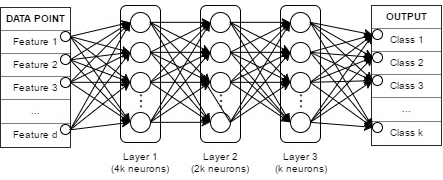
\includegraphics[scale=0.5]{NeuralNet/Network} \\
			\captionof{figure}{Architecture of our network.}
			\label{fig:nn_10_class_results}
		\end{center}
		The input data is randomly shuffled and split into training and testing datasets, with a ratio of \(9:1\). The model is trained for 50 epochs, using an Adaptive Gradient Descent (Adagrad) algorithm to fit and optimize weights throughout the model, with an initial learning rate \(\eta = 0.1\). Techniques are being considered that will decay the learning rate with relation to the loss calculated for each epoch.
		\par
		Displayed in Table \ref{table:nn_performance} and Figures \ref{fig:fig_nn_results_5} and \ref{fig:fig_nn_results_10} are the results of running the datasets through the current prototype network. Two different trials were run on each dataset, with the first trial learning and predicting against 5 classes of target values, and the second trial against 10 classes of target values. Each target class represents an equally sized partition of the data's target values. Predictions of a target class indicate that the given data point's sale price will fall within the boundaries that define that class's partition.
		\begin{center}
            \captionsetup{type=table}
			\begin{tabular}{r||c|c||c|c}
				& \multicolumn{2}{c||}{\small{5 classes}} & \multicolumn{2}{c}{\small{10 classes}} \\
				\hline 
				& \small{Train} & \small{Test} &  \small{Train} & \small{Test} \\
				\hline
				\small{Nashville} & \small{61.53\%} & \small{60.41\%} & \small{39.80\%} & \small{38.71\%} \\
				\hline
				\small{King County} & \small{51.92\%} & \small{51.92\%} & \small{30.90\%} & \small{29.94\%} \\
				\hline
				\small{Grand Rapids} & \small{57.05\%} & \small{56.34\%} & \small{33.74\%} & \small{32.75\%} \\
				\hline
			\end{tabular}
			\captionof{table}{Observed performance from neural network.}
			\label{table:nn_performance}
		\end{center}
		\begin{center}
            \captionsetup{type=figure}
			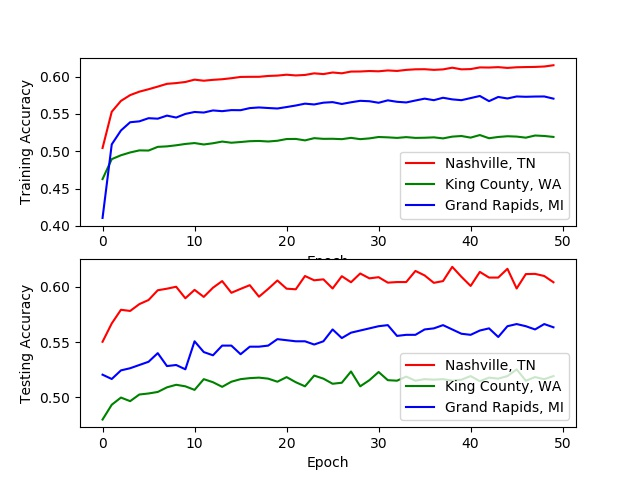
\includegraphics[scale=0.38]{NeuralNet/nn_5_class_results} \\
			\captionof{figure}{Results for classifying into 5 classes.}
			\label{fig:fig_nn_results_5}
		\end{center}
		\begin{center}
            \captionsetup{type=figure}
			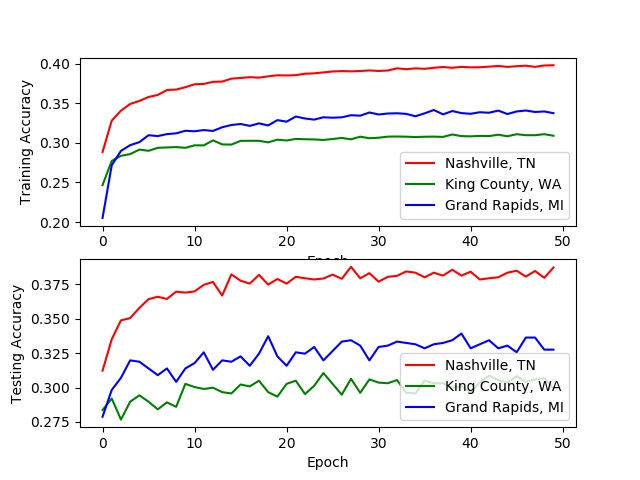
\includegraphics[scale=0.38]{NeuralNet/nn_10_class_results} \\
			\captionof{figure}{Results for classifying into 10 classes.}
			\label{fig:fig_nn_results_10}
		\end{center}
		The results show that the network performs better when classifying data points into a smaller number of target classes. Our goal from this point forward is to attempt to improve accuracy by investigating further improvements on preprocessing the input data, experimenting with different hyper-parameters for the network, and experimenting with varying network architectures. When accuracy improves, the goal with then be to increase the number of target classes in order to provide a more valuable estimation of the sales price of any given data point.
 		\section{Conclusion}
		We set out to look at how different machine learning approaches work when predicting or classifying home selling values.  We implmented models that included linear regression, logistic regression, decision trees, neural networks and ensemble methods. The methods themselves provided some interesting comparisons but one consistent thing we found with all models is the data the model is built on is one of the most important considerations.
		\par
		First processing the data for use by the models is extremely important. This includes cleaning up the data to a format the models handle well, such as splitting categorical features up into a binary category for each category in the feature. Additionaly filling holes in the data can significantly improve a model's ability to predict or classify data.
		\par
		Ultimately while there are things that can be done to get all of the information available from the data, a machine learning model is limited by how much information is actually in the data.  Table \ref{table:results} shows the results across the various models.  In all cases the Advanced Regression Techniques data performs the best.  This data is feature complete and has the largest number of features.  We believe this data was created specifically for developing machine learning models.  Of the remaining models, Nashville performs the worst as this data has the biggest holes in feature values, limiting the amount of actual information provided by the data.
		\begin{center}
	        \captionsetup{type=table}
			\begin{tabular}{r|c|c|c|c|c|c|c|c}
				& \small{Linear Regression} & \small{Linear Ensemble} &  \small{Logistic Regression} & \small{Logistic Ensemble} & \small{Decision Tree 1?} & \small{Decision Tree 2?} & \small{Neural Netork 1?} & \small{Neural Netork 2?}\\
				\hline 
				\small{Nashville} & \small{22.1e-03} & \small{N/A} & \small{N/A} & \small{N/A} & \small{?} & \small{?} & \small{?} & \small{?}\\
				\hline
				\small{Advanced Regression} & \small{1.8e-03} & \small{4.5e-03} & \small{1.7e-03} & \small{?} & \small{?} & \small{?} & \small{?} & \small{?}\\
				\hline
				\small{Redfin} & \small{6.3e-03} & \small{5.1e-03} & \small{8.5e-03} & \small{8.1e-03} & \small{?} & \small{?} & \small{?} & \small{?}\\
				\hline
				\small{King County} & \small{13.1e-03} & \small{13.1e-03} & \small{14.4e-03} & \small{13.2e-03} & \small{?} & \small{?} & \small{?} & \small{?}\\
				\hline
			\end{tabular}
			\captionof{table}{Combined Results.}
			\label{table:results}
		\end{center}
		\begin{thebibliography}{13}
			\bibitem{nashville_data}
			\textit{Nashville Housing Data: Home value data for the booming Nashville Market}
			Retrieved from \\ \small{\url{https://www.kaggle.com/tmthyjames/nashville-housing-data/}}
			
			\bibitem{kc_data}
			\textit{House Sales in King County, USA: Predict house price using regression}
			Retrieved from \\ \small{\url{https://www.kaggle.com/harlfoxem/housesalesprediction}}	
			
			\bibitem{kaggleblog}
			\textit{Data-driven property valuations: the real deal?}
			Retrieved from \\ \small{\url{http://blog.kaggle.com/2010/06/21/data-inc-are-avms-soothsayers-or-the-real-deal/}}
			
			\bibitem{scotsman}
			Schroeder, Steve.
			\textit{Fighting Fraud: A combination of collateral assessment and AVMs can maximize mortgage-fraud management}
			Retrieved from \\ \small{\url{http://www.scotsmanguide.com/Residential/Articles/2005/10/Fighting-Fraud/}}
			
			\bibitem{zillow}
			\textit{What is a Zestimate? Zillow's Home Value Forecast.}
			Retrieved from \\
			\small{\url{http://www.zillow.com/zestimate/}}
			
			\bibitem{lowrance}
			Lowrance, R. E. (2015).
			\textit{Predicting the Market Value of Single-Family Residential Real Estate}
			(Doctoral Dissertation). New York University. Retrieved from \small{\url{http://gradworks.umi.com/36/85/3685886.html}}
			
			\bibitem{park}
			Park, B., \& Bae, J. K. (2015).
			\textit{Using machine learning algorithms for housing price prediction: The case of Fairfax County, Virginia housing data.}
			Expert Systems with Applications, 42(6), 2928-2934. doi:10.1016/j.eswa.2014.11.040
			
			\bibitem{bin} 
			Bin, O. (2004).
			\textit{A prediction comparison of housing sales prices by parametric versus semi-parametric regressions.}
			Journal of Housing Economics, 13(1), 68-84. doi:10.1016/j.jhe.2004.01.001
			
			\bibitem{bourassa1} 
			Bourassa, S. C., Cantoni, E., \& Hoesli, M. (2010). 
			\textit{Predicting House Prices with Spatial Dependence: Impacts of Alternative Submarket Definitions.}
			SSRN Electronic Journal. doi:10.2139/ssrn.1090147
			
			\bibitem{bourassa2}
			Bourassa, S. C., Cantoni, E., \& Hoesli, M. (2007).
			\textit{Spatial Dependence, Housing Submarkets, and House Prices.}
			SSRN Electronic Journal. doi:10.2139/ssrn.771867
			
			\bibitem{kauko}
			Kauko, T., Hooimeijer, P., \& Hakfoort, J. (2002).
			\textit{Capturing Housing Market Segmentation: An Alternative Approach based on Neural Network Modelling.}
			Housing Studies, 17(6), 875-894. doi:10.1080/02673030215999
			
			\bibitem{azadeh} 
			Azadeh, A., Ziaei, B., \& Moghaddam, M. (2012).
			\textit{A hybrid fuzzy regression-fuzzy cognitive map algorithm for forecasting and optimization of housing market fluctuations.}
			Expert Systems with Applications, 39(1), 298-315. doi:10.1016/j.eswa.2011.07.020
			
			\bibitem{fan}
			Fan, G., Ong, S. E., \& Koh, H. C. (2006).
			\textit{Determinants of House Price: A Decision Tree Approach.}
			Urban Studies, 43(12), 2301-2315. doi:10.1080/00420980600990928
		\end{thebibliography}
	\end{multicols}
\end{document}
